\documentclass[12px, a4paper]{article}
\usepackage[margin=50pt]{geometry}
\usepackage{graphicx}
\graphicspath{ {./images} }
\title{Preserving Accents in Real-Time Audio Translation: A Novel Approach for Linguistic Fidelity}
\author{Irfan Wani - Lovely Professional University}
\begin{document}    
\maketitle
    \begin{abstract}
    Our system takes the audio as input and translates it into the target language in real-time. Audio files can also be used as input for the program and it will provide the reuslt in the desired language. The system is based on the concept of real-time audio translation. The system works in multiple steps, starting with taking the input from the user (primarily in english or detecting the language of the audio), converting the audio to text, taking the target language as the input from the user (like Hindi, Arabic etc) and then translating the text to the target language. Another step is the reverse of the previous steps where the text is converted back to audio and then played on the device.  NLP (Natural Language Processing) comes into play to make the whole thing working. NLP helps in translation, where it checks the grammer, words etc to make sure the translated text makes sense.
    The last step utilizes text-to-speech (TTS) models. These models are trained on audio recordings of different people speaking with different voices and tones, along with the corresponding input text. These models learn the characteristics of a particular voice, like pitch, timbre, and inflection. Then, when we provide some different text as input, they can synthesize speech that sounds like the target voice. Some AI systems can even adjust the synthesized speech to match the emotional tone of the original audio.
    \end{abstract}
    \textbf{Keywords: } NLP, Real-Time Audio Translation, Accents, Linguistic Fidelity, Google Translator AI, Whisper AI, Text-To-Speech.
\section{Introduction}
Talking about the realtime audio translation, it is a process where the audio is converted to text and then the text is translated to the target language. The process is done in real-time and the user can speak in the target language and the system will translate it to the target language. It is used in different fields like audio translation apps, language learning apps, audio caption generators etc. The input can be from a user in real time or from an audio file. The different steps involved in the process are:
\begin{enumerate}
    \item Taking the input from the user in realtime or using an input audio file. In this project, speech recognition package has been used to either read an audio file or to take the input from the user in real time by using the Microphone() class.
    \item Detecting the audio language. Speech recognition package has support for multiple models to detect the language of the audio. In this project, the model used is the Whisper model by Open AI.
    \item Converting the audio to text. The audio is converted to text using the Whisper model.
    \item Destination language is taken from the user to which the input audio will be translated. This is done by the same process.
    \item Using the Translator from googletrans package which provides the free Google Translation API for python, the input text is translated to the target language.
    \item Google Text to Speech is used to create an audio file which contains the translated text in the desired language.
    \item The audio file is played on the device using the playaudio package.
    \item  Text-to-speech (TTS) models are utilized that are trained on audio recordings of different speeches, along with the corresponding text. After learning different characteristics of the speeches, these models try to synthesize speech that sounds like the target voice. Some AI systems can even adjust the synthesized speech to match the emotional tone of the original audio.
    
    \textbf{Model used:}
    The model used in this project is Whisper AI from Open AI. Whisper is a general-purpose speech recognition model. It is trained on a large dataset of diverse audio and is also a multitasking model that can perform multilingual speech recognition, speech translation, and language identification.
\end{enumerate}
\section{Literature Review}
In current time, Real-time audio translation has become increasingly prevalent with the rise of globalization and the latest technologies. The ability to translate spoken language, especially in real-time, has revolutionized communication across geographical and linguistic barriers. 

Core Components of Audio Translation are:

\textbf{Automatic Speech Recognition (ASR)}: This technology converts spoken audio into text format. ASR systems are trained on vast amounts of speech data to recognize phonemes (basic units of sound) and translate them into words. Accuracy is crucial for effective translation, as errors in ASR can significantly impact the final output. Recently, the speech community is seeing a significant trend of moving from deep neural network based hybrid modeling to end-to-end modeling (often read as E2E modeling) for automatic speech recognition (ASR). While E2E models achieve the state-of-the-art results in most benchmarks in terms of ASR accuracy, hybrid models are still used in a large proportion of commercial ASR systems at the current time. There are lots of practical factors that affect the production model deployment decision. Traditional hybrid models, being optimized for production for decades, are usually good at these factors. (e.g., [Jinyu Li] (2021))

\textbf{Machine Translation (MT)}: This technology translates text from one language to another. Statistical or neural MT models analyze the source text, considering grammar, syntax, and context, to generate the target language translation. The quality of MT models significantly impacts the fluency and accuracy of the translated audio. Large Language Models (LLM) have demonstrated their strong ability in the field of machine translation (MT), yet they suffer from high computational cost and latency. Therefore, transferring translation knowledge from giant LLMs to medium-sized machine translation models is a promising research direction. However, traditional knowledge distillation methods do not take the capability of student and teacher models into consideration, therefore repeatedly teaching student models on the knowledge they have learned, and failing to extend to novel contexts and knowledge. (e.g., [Jiahuan Li, Shanbo Cheng, Shujian Huang, Jiajun Chen] (2024))

\textbf{Text-to-Speech (TTS)}: This technology synthesizes speech from written text. TTS systems are trained on audio recordings of human speech paired with corresponding text. They learn the characteristics of human voice, such as pitch, intonation, and rhythm, to generate natural-sounding speech in the target language. Non-autoregressive text to speech (TTS) models such as FastSpeech can synthesize speech significantly faster than previous autoregressive models with comparable quality. (e.g., [Yi Ren, Chenxu Hu, Xu Tan, Tao Qin, Sheng Zhao, Zhou Zhao, Tie-Yan Liu] (2021)) \linebreak\linebreak
\textbf{Recent Advancements}

\textbf{End-to-End Speech-to-Speech Translation (ST)}: This approach combines ASR, MT, and TTS into a single system, streamlining the translation process. Recent research by [Biao Zhang, Barry Haddow, Rico Sennrich] (2022) demonstrates promising results in terms of efficiency and fluency.

\textbf{Neural Machine Translation (NMT)}: NMT models utilize deep learning architectures to achieve superior translation accuracy compared to traditional statistical methods. Research by [Dzmitry Bahdanau, Kyunghyun Cho, Yoshua Bengio] (2016) explores the application of NMT for audio translation, achieving significant improvements in fluency and grammatical correctness. Neural machine translation is a recently proposed approach to machine translation. Unlike the traditional statistical machine translation, the neural machine translation aims at building a single neural network that can be jointly tuned to maximize the translation performance. The models proposed recently for neural machine translation often belong to a family of encoder-decoders and consists of an encoder that encodes a source sentence into a fixed-length vector from which a decoder generates a translation.

\textbf{Speaker Diarization and Adaptation}: These techniques identify and separate speech from different speakers within an audio recording. This allows for speaker-specific translation, particularly beneficial in conference settings. [Tae Jin Park, Naoyuki Kanda, Dimitrios Dimitriadis, Kyu J. Han, Shinji Watanabe, Shrikanth Narayanan] (2021) propose a diarization-based approach for real-time multi-speaker translation. Speaker diarization is a task to label audio or video recordings with classes that correspond to speaker identity, or in short, a task to identify "who spoke when". In the early years, speaker diarization algorithms were developed for speech recognition on multispeaker audio recordings to enable speaker adaptive processing. These algorithms also gained their own value as a standalone application over time to provide speaker-specific metainformation for downstream tasks such as audio retrieval. More recently, with the emergence of deep learning technology, which has driven revolutionary changes in research and practices across speech application domains, rapid advancements have been made for speaker diarization. \linebreak\linebreak

\begin{figure}[!htb]
    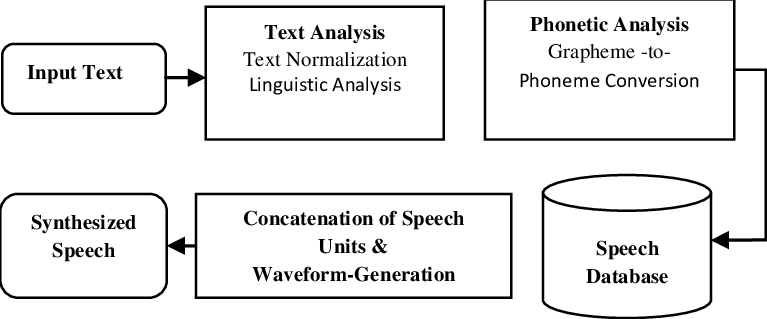
\includegraphics[width=\textwidth]{texttospeech.png}
    \caption{Block diagram of Text-to-Speech System Techniques of speech synthesis}
\end{figure}

\textbf{Challenges and Future Directions}

\textbf{Accuracy and Fluency}: Balancing accuracy in meaning preservation with natural-sounding fluency remains a challenge. Future research should focus on improving the robustness of ASR and NMT models to handle diverse speaking styles and background noise.

\textbf{Preserving Speaker Identity}: Current systems often lose speaker-specific characteristics like accent and intonation during translation. Research by [Sameen Maruf, André F. T. Martins, Gholamreza Haffari] (2019) explores accent-aware NMT to preserve speaker identity, paving the way for more nuanced translations. Despite the progress made in sentence-level NMT, current systems still fall short at achieving fluent, good quality translation for a full document. Recent works in context-aware NMT consider only a few previous sentences as context and may not scale to entire documents. To this end, they propose a novel and scalable top-down approach to hierarchical attention for context-aware NMT which uses sparse attention to selectively focus on relevant sentences in the document context and then attends to key words in those sentences. They also propose single-level attention approaches based on sentence or word-level information in the context. The document-level context representation, produced from these attention modules, is integrated into the encoder or decoder of the Transformer model depending on whether we use monolingual or bilingual context. The performed experiments and evaluation on English-German datasets in different document MT settings show that the selective attention approach not only significantly outperforms context-agnostic baselines but also surpasses context-aware baselines in most cases.

\textbf{Real-Time Performance}: Ensuring accurate and fluent translation while maintaining real-time processing speed is crucial for practical applications. Optimizing algorithms and utilizing powerful hardware are key areas for future development. Such features can be integrated with most of the streaming platforms these days, if working properly. With such models in action, any video can be translated into another language in real-time, maintaining the identity, accent and emotions of the person in the video.

\begin{figure}[!htb]
    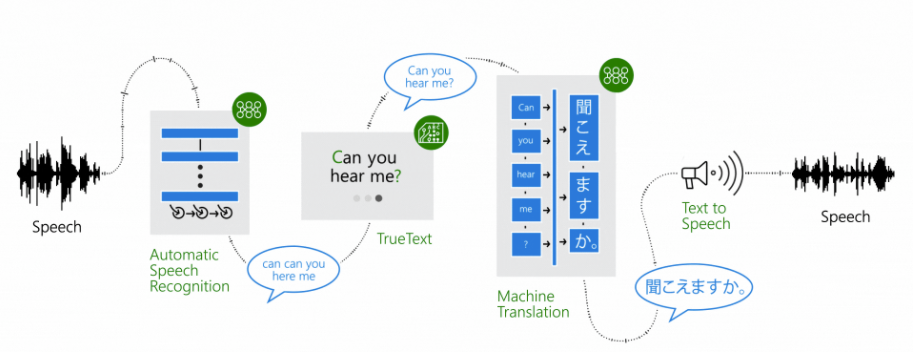
\includegraphics[width=\textwidth]{audiotrans.png}
    \caption{Real-time speech translation}
\end{figure}

\newpage
\section{Methodology}
Audio Translation mainly includes two steps: Speech Recognition, using Automatic Speech Recognition System (ASR) and Machine Translation.

\textbf{Automatic Speech Translation:} In this project, Whisper AI (from Open AI) is used which is an Automatic Speech Translation system. It has been trained on a large dataset of more than 650k hours of speeches of different people with different languages and accents.

\begin{figure}[!htb]
    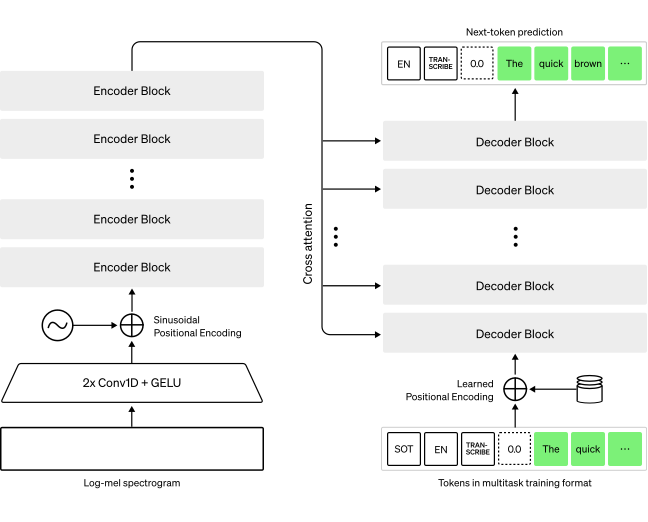
\includegraphics[width=\textwidth]{whisper1.png}
    \caption{Architecture of Whisper AI}
\end{figure}

The Whisper architecture is a simple end-to-end approach. It is implemented as an encoder-decoder Transformer where the input audio is split into 30-second chunks (parts), then converted into a log-Mel spectrogram, and atlast, it is passed into an encoder. A decoder is trained to predict the corresponding text caption which performs the processing along with the steps like, intermixing of special tokens that direct the single model to perform tasks such as language identification, phrase-level timestamps, multilingual speech transcription, and Translation of speech to English language.

\begin{figure}[!htb]
    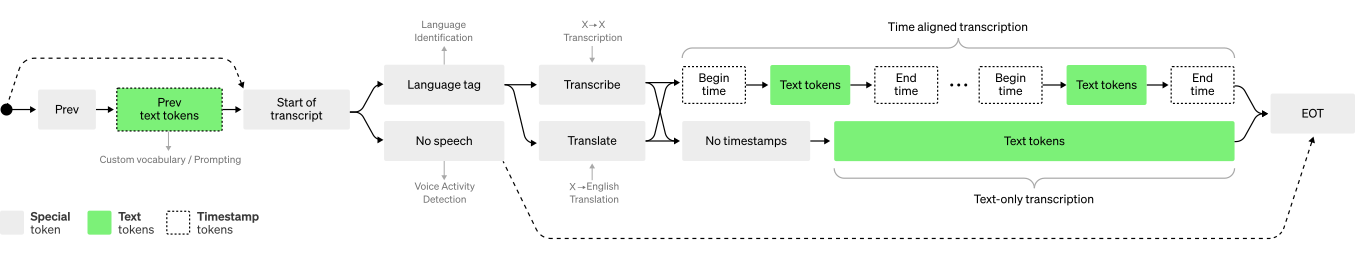
\includegraphics[width=\textwidth]{asr-details.png}
    \caption{Working of Automatic Speech Recognition(ASR)}
\end{figure}

\textbf{Available models and languages in Whisper AI:}
There are five model sizes, four of which are English-only versions which offer speed and accuracy tradeoffs. Below are the names of the available models and their approximate memory requirements and inference speed relative to the large model. Actual speed may vary depending on many factors like the available hardware etc.

\begin{table}[!h]
    \centering
    \begin{tabular}{|c|c|c|c|c|c|}
        \hline
        \textbf{Size} & \textbf{Parameters} & \textbf{English-only model} & \textbf{Multilingual model} & \textbf{Required VRAM} & \textbf{Relative speed}\\
        \hline
        tiny & 39 M & tiny.en & tiny & ~1 GB & ~32x\\
        \hline
        base & 74 M & base.en & base & ~1 GB & ~16x\\
        \hline
        small & 244 M & small.en & small & ~2 GB & ~6x\\
        \hline
        medium & 769 M & medium.en & medium & ~5 GB & ~2x\\
        \hline
        large & 1550 M & N/A & large & ~10 GB & 1x\\
        \hline
    \end{tabular}
\end{table}


\section{Results and Discussion}
\section{Future Scope}
\section{Conclusion}
\section{References}
\begin{enumerate}
    \item Jinyu Li - Recent Advances in End-to-End Automatic Speech Recognition [https://arxiv.org/abs/2111.01690]
    \item Whisper AI [https://github.com/openai/whisper]
    \item Alec Radford, Jong Wook Kim, Tao Xu,  Greg Brockman,  Christine McLeavey, Ilya Sutskever - Robust Speech Recognition via Large-Scale Weak Supervision [https://arxiv.org/pdf/2212.04356.pdf]
    \item Jiahuan Li, Shanbo Cheng, Shujian Huang, Jiajun Chen - MT-PATCHER: Selective and Extendable Knowledge Distillation from Large Language Models for Machine Translation [https://arxiv.org/abs/2403.09522/]
    \item Dzmitry Bahdanau, Kyunghyun Cho, Yoshua Bengio - Neural Machine Translation by Jointly Learning to Align and Translate
    [https://arxiv.org/abs/1409.0473/]
\end{enumerate}
\end{document}